\begin{figure}[htbp]
	\centering
	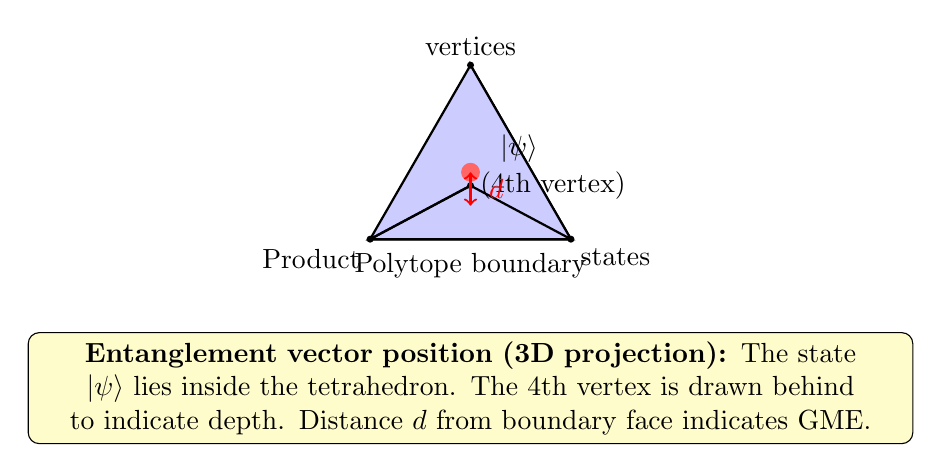
\begin{tikzpicture}[scale=0.85]
		\draw[thick, fill=blue!10] (0,0) -- (3,0) -- (1.5,2.6) -- (1.5,0.8) -- cycle;
		\draw[thick, fill=blue!20] (0,0) -- (3,0) -- (1.5,2.6) -- cycle;
		\draw[thick, fill=blue!20] (0,0) -- (3,0) -- (1.5,0.8) -- cycle;
		\draw[thick] (0,0) -- (1.5,0.8);

		\fill[red!60] (1.5,1.0) circle (4pt);
		\node[above right] at (1.8,1.0) {$|\psi\rangle$};

		\fill (0,0) circle (1.5pt) node[below left] {Product};
		\fill (3,0) circle (1.5pt) node[below right] {states};
		\fill (1.5,2.6) circle (1.5pt) node[above] {vertices};
		\fill (1.5,0.8) circle (1.5pt) node[right] {(4th vertex)};

		\draw[<->, thick, red] (1.5,0.5) -- (1.5,1.0) node[midway, right=3pt] {$d$};

		\node at (1.5,-0.4) {Polytope boundary};

		\node[draw, rounded corners, fill=yellow!20, text width=11cm, align=center, below=0.5cm] at (1.5,-0.8) {
			\textbf{Entanglement vector position (3D projection):} The state $|\psi\rangle$ lies inside the tetrahedron. The 4th vertex is drawn behind to indicate depth. Distance $d$ from boundary face indicates GME.
		};
	\end{tikzpicture}
	\caption{Entanglement polytope (3D projection) showing state $|\psi\rangle$ positioned within the tetrahedron. The 4th vertex behind the base indicates 3D depth.}
	\label{fig:entanglement-polytope-position-3d}
\end{figure}
